\documentclass[12pt]{book}
\newcommand{\mbf}[1]{\mbox{\boldmath$#1$}}
% definice zlomku
\newcommand{\del}[2]{\mbox{$\displaystyle\frac{#1}{#2}$}}
% definice prvni parcialni derivace funkce
\newcommand{\ppd}[2]{\del{\partial{#1}}{\partial{#2}}}
% definice druhe parcialni derivace funkce podle x a y
\newcommand{\dpd}[3]{\del{\partial^{2}\>\!\!{#1}}{\partial{#2}\ \partial{#3}}}
% definice n-te parcialni derivace funkce
\newcommand{\npd}[3]{\del{\partial^{#1}\>\!\!{#2}}{\partial{#3}^{#1}}}
% definice prvni derivace funkce
\newcommand{\od}[2]{\del{{\rm d}\>\!{#1}}{{\rm d}{#2}}}
% definice n-te obycejne derivace funkce
\newcommand{\nod}[3]{\del{{\rm d}^{#1}\>\!\!{#2}}{{\rm d}{#3}^{#1}}}
\usepackage{makeidx}
\usepackage{graphicx}
\makeindex

\setcounter{secnumdepth}{4}
\setcounter{totalnumber}{4}
\oddsidemargin=5mm
\evensidemargin=5mm
\textwidth=160mm
\topmargin=-2.0cm
\textheight=250mm
\headheight=1.5cm


\begin{document}
\tableofcontents
\chapter {MESH GENERATORS MANUAL}

\section{INTRODUCTION}

In order to generate regular meshes on regular domains, simple mesh
generators are collected in the directory SIFEL/PREP.
There are mesh generators for single processor
computing as well as for the parallel computing.
The generators for single processor computing are located in the directory SIFEL/PREP/SEQMESHGEN.
The generators for parallel computing are located in the directory SIFEL/PREP/PARMESHGEN. 
All generators use SIFEL format, thus the switch 0 should be used
in the preprocessor file (mechprep, transprep).


\section {2D GENERATORS}

2D generators gnerate rectangular domain with regular mesh. User may enter
number of elements in the x and y direction and length and height of domain.
All nodes on the boundaries have assigned extra property number so the nodes
on the left boundary have assigned property number 0, nodes on the top boundary
have assigned property number 1, nodes on the right boundary have assigned
property number 2 and nodes on the bottom boundary have assigned property
number 3. Rest of nodes have assigned property number 4.
User may enter whether generator should print edge numbers on the elements.
Edge numbers are used in case that user would like to use edge load oon the elements
(MEFEL) or heat flux or heat transfer (TRFEL). The user have to set up
read\_edge\_number switch to the vlaue 1 in the preprocessor file (mechprep, transprep).
Edge on the left has number 1, on the top has number 2, on the right has number 3 and
on the bottom has number 4.\\
\\
Usage of each program is :\\
\\
program\_name param1 param2 param3 param4 param5 param6\\
\\
where :
\begin{itemize}
\item param1 is output file name
\item param2 is length in the x direction
\item param3 is height in the y direction
\item param4 is number of elements in the x direction
\item param5 is number of elements in the y direction
\item param6 is switch which controls whether edge numbers on the elements are printed
          (0 = not print, 1 = print)
\end{itemize}
The following programs is possible to use :
\begin{itemize}
\item gensifquad.cpp  - this program generates mesh with quadrilateral elements (linear aproximation).
\item gensifquadq.cpp - this program generates mesh with quadrilateral elements (quadratic aproximation).
\item gensiftria.cpp  - this program generates mesh with triangle elements (linear aproximation)
\end{itemize}

\section {3D generators}

\subsection {gensifhex.cpp}

(this generator produces the new format of *.top files)

This generator generates regular mesh of hexagonal elements with linear approximation functions
on rectangular parallelepiped domain.
\\
Syntax is the following:
\\
gensifhex param1 param2 param3 param4 param5 param6 param7\\
\\
where :\\
\begin{itemize}
\item param1 is output file name
\item param2 is the length in  $x$ direction
\item param3 is the length in  $y$ direction
\item param4 is the length in  $z$ direction
\item param5 is the number of elements in $x$ direction
\item param6 is the number of elements in $y$ direction
\item param7 is the number of elements in $z$ direction
\end{itemize}

\begin{table}
\begin{center}
\begin{tabular}{|c|c|}
\hline
vertex & property
\\ \hline
1 & 1
\\ \hline
2 & 2
\\ \hline
3 & 3
\\ \hline
4 & 4
\\ \hline
5 & 5
\\ \hline
6 & 6
\\ \hline
7 & 7
\\ \hline
8 & 8
\\ \hline
\end{tabular}
\caption{Vertex properties.}
\end{center}
\end{table}

\begin{table}
\begin{center}
\begin{tabular}{|c|c|c|}
\hline
edge number & edge nodes & property
\\ \hline
1 & 1, 2 & 1
\\ \hline
2 & 2, 3 & 2
\\ \hline
3 & 3, 4 & 3
\\ \hline
4 & 4, 1 & 4
\\ \hline
5 & 5, 6 & 9
\\ \hline
6 & 6, 7 & 10
\\ \hline
7 & 7, 8 & 11
\\ \hline
8 & 8, 5 & 12
\\ \hline
9 & 1, 5 & 5
\\ \hline
10 & 2, 6 & 6
\\ \hline
11 & 3, 7 & 7
\\ \hline
12 & 4, 8 & 8
\\ \hline
\end{tabular}
\caption{Edge properties.}
\end{center}
\end{table}

\begin{table}
\begin{center}
\begin{tabular}{|c|c|c|}
\hline
surface number & surface nodes& property
\\ \hline
1 & 1, 4, 8, 5 & 1
\\ \hline
2 & 2, 1, 5, 6 & 2
\\ \hline
3 & 3, 2, 6, 7 & 3
\\ \hline
4 & 4, 3, 7, 8 & 4
\\ \hline
5 & 1, 2, 3, 4 & 5
\\ \hline
6 & 5, 6, 7, 8 & 6
\\ \hline
\end{tabular}
\caption{Surface properties.}
\end{center}
\end{table}

\subsection {gensifhexq.cpp}

This generator generates prism or tube domain with regular mesh with hexagonal elements (quadratic aproximation).
Behaviour is similar as 2D generators, but edge numbers are not printed and properties of nodes are
assigned following way:\\
Nodes with x coordinate x = 0 has assigned property number 0, rest of nodes has assigned property number 1\\
Usage of each program is :\\
\\
program\_name 1 param1 param2 param3 param4 param5 param6 param7\\
\\
generates prism where :
\begin{itemize}
\item param1 is output file name
\item param2 is length in the x direction
\item param3 is length in the y direction
\item param4 is length in the z direction
\item param5 is number of elements in the x direction
\item param6 is number of elements in the y direction
\item param7 is number of elements in the z direction
\end{itemize}
program\_name 2 param1 param2 param3 param4 param5 param6 param7 param8\\
\\
generates tube where :
\begin{itemize}
\item param1 is output file name
\item param2 is radius
\item param3 is length
\item param4 is thick
\item param5 is number of elements in the radius direction
\item param6 is number of elements in the length direction
\item param7 is number of elements in the thick direction
\item param8 is angel of tube segment.
\end{itemize}

\section{Parallel 2D generators}

\subsection{pargenquad.cpp}

 This generator produces similar mesh as the gensifquad, but divides rectangular domain to given
number of rectangular subdomains. In addition program generates preprocessor files.
Domain will have on the left edge supports and the right edge will be loaded with given load.
Positive global node numbers are assigned  only on the edges between subdomains. Nodes inside subdomians
have assigned zero.\\
 Input for this program is data file with folowing structure :
\begin{itemize}
\item $Ndx$    = number of rectangular subdomains in the x direction
\item $Ndy$    = number of rectangular subdomains in the y direction
\item $dimx_1$ = length of 1. subdomain in the x direction
\item $nex_1$  = number of generated elements of 1. subdomain in the x direction\\
.\\
.\\
.\\
\item $dimx_{ndx}$ = length of ndx-th subdomain in the x direction
\item $nex_{ndx}$  = number of generated elements of ndx-th subdomain in the x direction
\item $dimy_1$   = length of 1. subdomain in the y direction
\item $ney_1$    = number of generated elements of 1. subdomain in the y direction\\
.\\
.\\
.\\
\item $dimy_{ndy}$  = length of ndy-th subdomain in the y direction
\item $ney_{ndy}$   = number of generated elements of ndy-th subdomain in the y direction
\item $ofname$    = name of output files wtihout any extension, program automatically adds numbers to file names and
            extension .top for the topology and .pr for the preprocessor file
\item $auxfname$  = name of auxiliary file for the nonlinear statics
\item $tmplfname$ = name of template preprocessor file. Structure of the file will be described later
\item $Edgn$      = Switch for output Edge numbers in the topology file. Set to value 0 when edge numbers shouldn't be printed.
            set to value 1 when edge numbers should be printed. Edge numbers are used togeather with elements with edge load.
            So value 1 is usually used when the template file conatains edge load.
\item $Ndofn$     = number of dofs in nodes
\item $f_{1,1}$      = value of force load in the 1. direction for load case 1\\
.\\
.\\
.\\
\item $f_{nodfn,1}$  = value of force load in the ndofn-th direction for load case 1\\
.\\
.\\
.\\
.\\
.\\
\item $f_{1,n}$      = value of force load in the 1. direction for load case n\\
.\\
.\\
.\\
\item $f_{nodfn,n}$  = value of force load in the ndofn-th direction for load case n
\end{itemize}
Number of load cases is specified in the template file.

Example of data file :

Given rectangular domain with dimension 34 units in the x direction
and 8 units in the y direction. It should be divided to the 2 subdomains
in each direction. Each subdomain should be divided by the regular mesh to
the 4 elements, 2 elements in the each direction.


Data file looks like follow :\\
\\
{\it
2 2\\
14 2\\
20 2\\
4  2\\
4  2\\
MYEXAM/exam\\
DATA/graph\\
templex\\
0\\
2\\
-100.0 0.0\\
\\
}
%Subdomain numbering :
\begin{figure}[h]
\includegraphics[width=120mm]{pgquaddn.eps}
\end{figure}
%Element numbering :
\begin{figure}
\includegraphics[width=120mm]{pgquaden.eps}
\end{figure}
%Local node numbering :
\begin{figure}
\includegraphics[width=120mm]{pgquadlnn.eps}
\end{figure}
%Global node numbering :
\begin{figure}
\includegraphics[width=120mm]{pgquadgnn.eps}
\end{figure}
%Boundary condition :
\begin{figure}
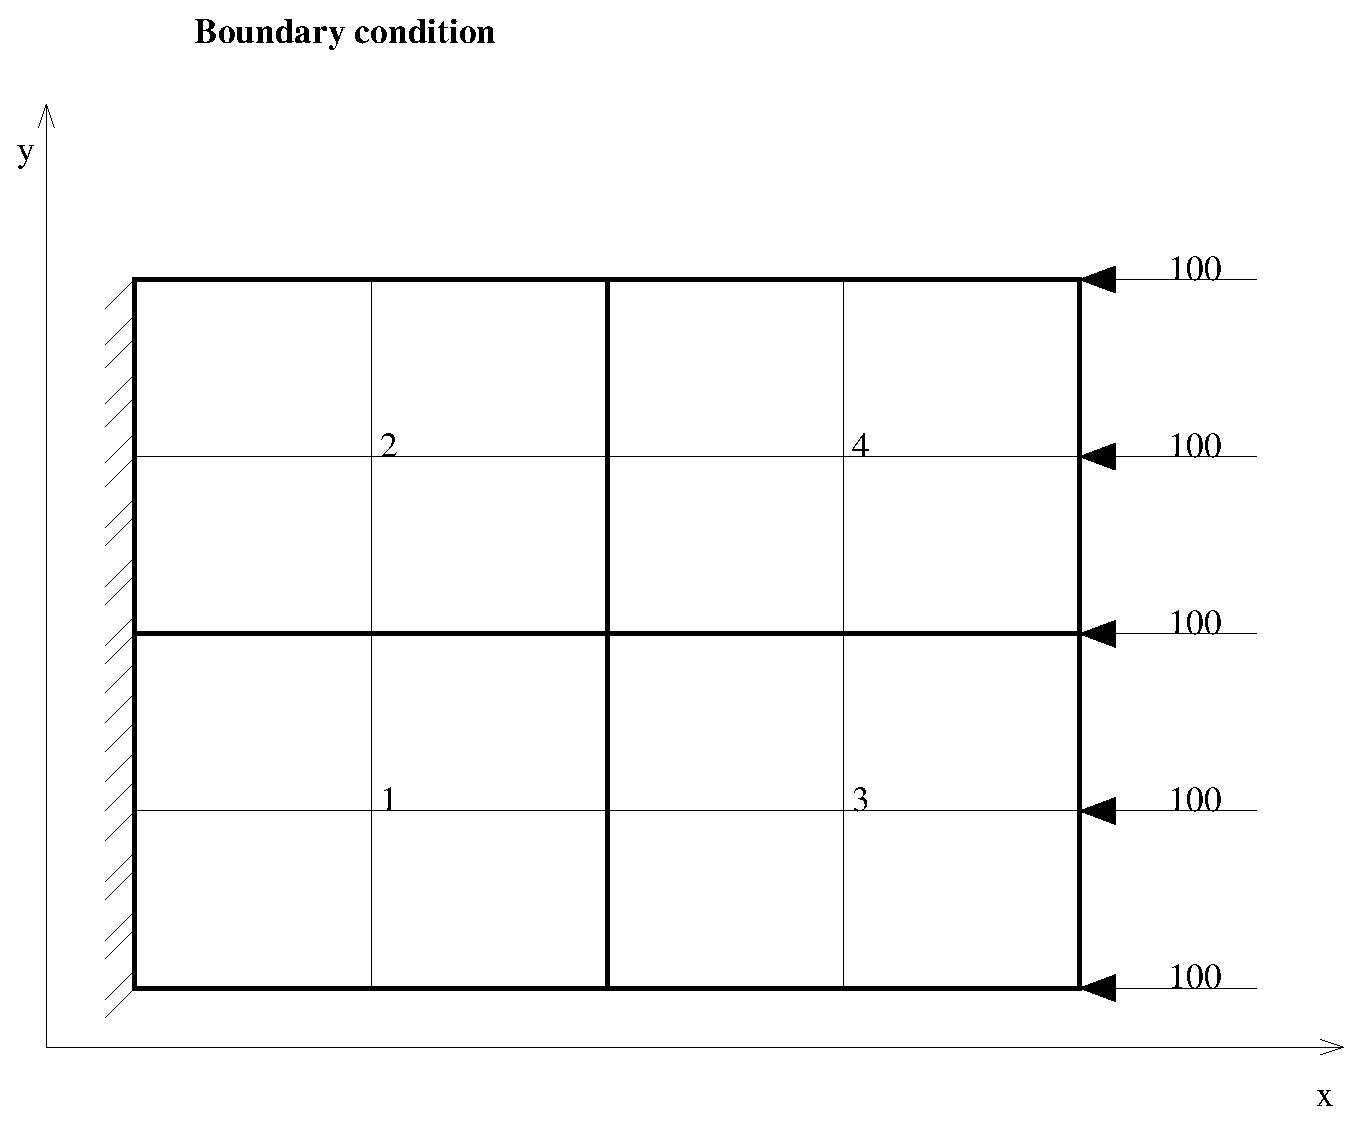
\includegraphics[width=120mm]{pgquadbc.eps}
\end{figure}
\\
\subsubsection{Template preprocessor file}
This file is used for generating preprocessor files for each subdomain. It contains all common
data about subdomains. For example problem description, number of load cases, materials, cross-section, load.
pargenquad only assigns boundary conditions for subdomains.\\
\\
Example of template preprocessor file :\\
{\it
dbmat\#             file with database of materials\\
dbcrs\#             file with database of cross-sections\\
begin\\
\# Here is problem desciption\\
Muj job\\
1\\
1\\
0 0 0 0 0 0\\
1 1\\
end\\
1  \#number of load cases\\
begin\\
\# This section assigns nodal properties common for each subdomain\\
\# property 1 = nodes on the lef edge\\
\# property 2 = nodes between lef and right edges\\
\# property 3 = nodes on the right edge\\
1 ndofn 2\\
1 crsec 10 1\\
2 ndofn 2\\
2 crsec 10 1\\
3 ndofn 2\\
3 crsec 10 1\\
end\\
\\
begin\\
\# This section assigns element properties common for each subdomain\\
\# Each element has property 0.\\
0 eltype 5 21 10\\
0 sscomp 5 1\\
0 mater 1 1 1\\
end\\
}

\subsection{pargenbrick.cpp}

Same as pargenquad but it divides 3D prism domain to given number of prism subdomains.
Global node numbers are numbered in the same way as the pargenquad. It means on the common edges
between subdomains are generated positive global node numbers else global node number is zero.
The first are generated subdomains in the z direction, then are generated in the y direction and
then in the x direction. Elements are generated in the same way as subdomains.\\
\\
Input for this program is data file with folowing structure :\\
\begin{itemize}
\item $Ndx$    = number of rectangular subdomains in the x direction
\item $Ndy$    = number of rectangular subdomains in the y direction
\item $Ndz$    = number of rectangular subdomains in the z direction
\item $dimx_1$ = length of 1. subdomain in the x direction
\item $nex_1$  = number of generated elements of 1. subdomain in the x direction\\
.\\
.\\
.\\
\item $dimx_{ndx}$ = length of ndx-th subdomain in the x direction
\item $nex_{ndx}$  = number of generated elements of ndx-th subdomain in the x direction
\item $dimy_1$   = length of 1. subdomain in the y direction
\item $ney_1$    = number of generated elements of 1. subdomain in the y direction\\
.\\
.\\
.\\
\item $dimy_{ndy}$  = length of ndy-th subdomain in the y direction
\item $ney_{ndy}$   = number of generated elements of ndy-th subdomain in the y direction
\item $dimz_1$   = length of 1. subdomain in the z direction
\item $nez_1$    = number of generated elements of 1. subdomain in the z direction\\
.\\
.\\
.\\
\item $dimz_{ndz}$  = length of ndz-th subdomain in the z direction
\item $nez_{ndz}$   = number of generated elements of ndz-th subdomain in the z direction
\item $ofname$    = name of output files wtihout any extension, program automatically adds numbers to file names and
            extension .top for the topology and .pr for the preprocessor file
\item $auxfname$  = name of auxiliary file for the nonlinear statics
\item $tmplfname$ = name of template preprocessor file. Structure of the file will be described later
\item $fx_1$      = value of force load in the x direction for load case 1
\item $fy_1$      = value of force load in the y direction for load case 1
\item $fz_1$      = value of force load in the z direction for load case 1\\
.\\
.\\
.\\
.\\
.\\
\item $fx_{nlc}$    = value of force load in the x direction for load case nlc
\item $fy_{nlc}$    = value of force load in the y direction for load case nlc
\item $fz_{nlc}$    = value of force load in the z direction for load case nlc
\end{itemize}

\subsection {pargenquadd.cpp, pargenbrickd}

Programs are same as pargenquad and pargenbrick but global node numbering is
modificated for DP-FETI. So the nodes on the common edges have assigned positive global numbers and
nodes in the common corners of subdomains have assigned negative global numbers.


\subsection {pargenquadt.cpp}

Program is same as the pargenquad but it has been modified for PARTRFEL. The modification lies in the
boundary condition. Input file has ame format but section with load was replaced with section of
boundary condition. Template preprocessor file should be in the TRFEL preprocessor format. Number of load
cases this time means number of transported media.
Here is example of input file domain divided to the 12 subdomains
(4 in the x direction and 3 in the y direction) :\\
\\
{ \it
4 3\\
0.125 38\\
0.125 38\\
0.125 38\\
0.125 38\\
0.166666666666 50\\
0.166666666666 50\\
0.166666666666 50\\
rbrno\\
EXAM/rbrno\\
templ4pddds\\
1\\
0.007639 0.012857\\
290.0 290.0\\
}
\\
The last two lines contain boundary condition for the first and second transported medium

\subsection {pargentria.cpp and pargentriad.cpp}

Programs are same as the pargenquad and pargenquadd but they genrate linear tringles instead of quadrilaterals.
Input file format is same as in the pargenquad(d).

\end{document}